% !TeX document-id = {0be8c18c-9430-4e9a-bdd9-12beadebfebc}
% !TeX TXS-program:bibliography = txs:///biber
\documentclass[11pt]{beamer}

\usepackage[brazilian]{babel}

\uselanguage{portuguese}
\languagepath{portuguese}
\deftranslation[to=portuguese]{Theorem}{Teorema}
\deftranslation[to=portuguese]{theorem}{teorema}
\deftranslation[to=portuguese]{Example}{Exemplo}
\deftranslation[to=portuguese]{example}{exemplo}
\deftranslation[to=portuguese]{Lemma}{Lema}
\deftranslation[to=portuguese]{lemma}{Lema}
\deftranslation[to=portuguese]{Corollary}{Corolário}
\deftranslation[to=portuguese]{corollary}{corolário}
%\deftranslation[to=portuguese]{and}{e}


\usepackage[utf8]{inputenc}
\usepackage[T1]{fontenc}
\usepackage{lmodern}
\usepackage{amsmath}
\usepackage{amssymb}
\usepackage{mathtools}
\usepackage{color}
\usepackage{pgfplots}
\usepackage{tikz}
\usepackage{subcaption}
%\usepackage{appendixnumberbeamer}

\newenvironment{transitionframe}{
	\setbeamercolor{background canvas}{bg=yellow}
	\begin{frame}}{
	\end{frame}
}
\usetheme{default}
\usefonttheme{structuresmallcapsserif}

%% I use a beige off white for my background
\definecolor{MyBackground}{RGB}{255,253,218}
\useinnertheme[shadow]{rounded}
\setbeamercolor{block title}{bg=MyBackground}
\setbeamercolor{block body}{bg=MyBackground}
\setbeamercolor{example title}{bg=MyBackground}
\setbeamercolor{example body}{bg=MyBackground}


\newcommand{\blue}[1]{\textcolor{blue}{#1}}
\newcommand{\red}[1]{\textcolor{red}{#1}}
\newcommand{\purple}[1]{\textcolor{purple}{#1}}
\newcommand{\gray}[1]{\textcolor{gray}{#1}}
\setbeamertemplate{navigation symbols}{}
%\setbeamertemplate{page number in head/foot}[appendixframenumber]

%\usepackage{graphics}
\usepackage{graphicx}

\definecolor{blue_emph}{RGB}{0,114,178}
\definecolor{red}{RGB}{213,94,0}
\definecolor{yellow}{RGB}{240,228,66}
\definecolor{green}{RGB}{0,158,115}
\definecolor{purple}{RGB}{204,121,167}
\definecolor{orange}{RGB}{230,159,0}
\definecolor{lightblue}{RGB}{86,180,233}

%\setbeamercolor{frametitle}{fg=blue}
%\setbeamercolor{title}{fg=blue}
\setbeamertemplate{footline}[frame number]
\setbeamertemplate{navigation symbols}{} 
\setbeamertemplate{itemize items}{-}
%\setbeamercolor{itemize item}{fg=blue}
%\setbeamercolor{itemize subitem}{fg=blue}
\setbeamertemplate{enumerate items}[default]
%\setbeamercolor{enumerate subitem}{fg=blue}
\setbeamercolor{button}{bg=MyBackground,fg=blue}
\usefonttheme{structuresmallcapsserif}

%\setbeamercolor{section in toc}{fg=blue}
%\setbeamercolor{subsection in toc}{fg=red}
\setbeamersize{text margin left=1em,text margin right=1em} 


\usepackage{appendixnumberbeamer}

\usepackage[
backend=biber,
style=authoryear,
natbib=true
]{biblatex}
\addbibresource{../bibliography.bib}

\newenvironment{wideitemize}{\itemize\addtolength{\itemsep}{10pt}}{\enditemize}
\newenvironment{wideenumerate}{\enumerate\addtolength{\itemsep}{10pt}}{\endenumerate}
\newenvironment{halfwideitemize}{\itemize\addtolength{\itemsep}{0.5em}}{\enditemize}
\newenvironment{halfwideenumerate}{\enumerate\addtolength{\itemsep}{0.5em}}{\endenumerate}


\author{Luis A. F. Alvarez}
\title{EAE1223: Econometria III}
\subtitle{Aula 6 - Modelos vetoriais autorregressivos}
%\logo{}
%\institute{}
\date{\today}
%\subject{}
%\setbeamercovered{transparent}

\begin{document}

\begin{frame}[plain]
	\maketitle
\end{frame}

\begin{frame}{Vetores aleatórios e matriz de variância-covariância}
\begin{halfwideitemize}
	\item Um vetor (coluna) aleatório $\boldsymbol{X}$, com valores em $\mathbb{R}^d$, é uma função com domínio no espaço de probabilidade $(\Omega,\Sigma,\mathbb{P})$ e contradomínio em $\mathbb{R}^d$.
\begin{itemize}
	\item Posto de outra forma, um vetor aleatório  $\boldsymbol{X}$ é um vetor cujas entradas $\boldsymbol{X}_j$, $j=1\ldots, d$, são variáveis aleatórias com valores reais.
\end{itemize}
\item Para um vetor aleatório $\boldsymbol{X}$, a matriz de variância-covariância, $\mathbb{V}[\boldsymbol{X}]$, é definida como:

$$\mathbb{V}[\boldsymbol{X}]  = \mathbb{E}[\boldsymbol{X}\boldsymbol{X}'] - \mathbb{E}[\boldsymbol{X}]\mathbb{E}[\boldsymbol{X}']$$

\item Matriz de variância-covariância é $d \times d$, simétrica, positiva semidefinida, com entrada $(i,j)$ iguais a:

$$\mathbb{V}[\boldsymbol{X}]_{i,j}= \operatorname{cov}(\boldsymbol{X}_i,\boldsymbol{X}_j)\, .$$

\end{halfwideitemize}
\end{frame}

\begin{frame}{Matriz de covariância entre dois vetores aleatórios}
	\begin{itemize}
		\item Seja $\boldsymbol{X}$ um vetor aleatório em $\mathbb{R}^d$, e $\boldsymbol{Y}$ um vetor aleatório em $\mathbb{R}^p$, definimos a matriz de covariância entre $\boldsymbol{X}$ e $\boldsymbol{Y}$  como:
		
		$$\operatorname{cov}(\boldsymbol{X},\boldsymbol{Y}) = \mathbb{E}[\boldsymbol{X}\boldsymbol{Y}'] - \mathbb{E}[\boldsymbol{X}]\mathbb{E}[\boldsymbol{Y}'] \, .$$
		\item Matriz $d \times p$ em que a entrada $(i,j)$ é igual a:
		
		$$\operatorname{cov}(\boldsymbol{X},\boldsymbol{Y})_{i,j} = \operatorname{cov}(\boldsymbol{X}_i,\boldsymbol{Y}_j)$$
	\end{itemize}
\end{frame}

\begin{frame}{Processo vetorial fracamente estacionário}
\begin{itemize}
		\item Um processo estocástico vetorial é uma coleção de vetores aleatórios definidos em $\mathbb{R}^d$, indexados por um conjunto $\mathcal{I}$, isto é $\{\boldsymbol{X}_t: t \in \mathcal{I}\}$, onde cada $\boldsymbol{X}_t$ é vetor aleatório em $\mathbb{R}^d$.
		\begin{itemize}
			\item Cada entrada $j = 1\ldots d$ define um processo estocástico com valores reais $\{\boldsymbol{X}_{j,t}: t \in \mathcal{I}\}$ descrevendo a evolução da $j$-ésima entrada ao longo de $\mathcal{I}$.
		\end{itemize}
	\item Um processo estocástico vetorial $\{\boldsymbol{X}_t: t \in \mathcal{T}\}$ indexado no tempo $ \mathcal{T}$ é dito fracamente estacionário se:
	
	\begin{enumerate}
		\item$ \mathbb{E}[\boldsymbol{X}_t] = \boldsymbol{\mu}$ para todo $t \in \mathcal{T}$.
		\item $ \mathbb{V}[\boldsymbol{X}_t] = \Sigma_0$ para todo $t \in \mathcal{T}$, com $\operatorname{tr}(\Sigma_0) < \infty$.
		\item $\operatorname{cov}(\boldsymbol{X}_t,\boldsymbol{X}_{t-h}) = \Sigma_h$, para todo $t \in \mathcal{T}$, $h \in \mathcal{N}$.
	\end{enumerate}
	\item Extensão do conceito de série de tempo estacionária para o caso vetorial.
	\item Pedimos estabilidade das covariâncias contemporâneas e extemporâneas entre as entradas dos vetores.
	\item \textbf{Obs:} se processo vetorial é fracamente estacionário, cada uma das entradas $\{\boldsymbol{X}_{j,t}: t \in \mathcal{T}\}$ , $j =1,\ldots, d$, é fracamente estacionária.
\end{itemize}
\end{frame}

\begin{frame}{Ruído branco vetorial}
	\begin{itemize}
		\item Um processo estocástico vetorial  $\{\boldsymbol{X}_t: t \in \mathcal{T}\}$ com valores em $\mathbb{R}^d$ é dito um ruído branco vetorial se:
		
		\begin{itemize}
			\item $\mathbb{E}[\boldsymbol{X}_t] = \boldsymbol{0}_{d\times 1}$, para todo $t \in \mathcal{T}$.
		\item $ \mathbb{V}[\boldsymbol{X}_t] = \Sigma_0$ para todo $t \in \mathcal{T}$, com $\operatorname{tr}(\Sigma_0) < \infty$.
\item $\operatorname{cov}(\boldsymbol{X}_t,\boldsymbol{X}_{l}) = \boldsymbol{0}_{d\times d}$, para todo $t \neq l$.
		\end{itemize}
		\item No ruído branco vetorial, permitimos associação contemporânea entre as entradas do vetor, mas não há nem autodependência nem dependência cruzada entre as entradas no tempo.
	\end{itemize}
\end{frame}

\begin{frame}{Ruído branco vetorial Gaussiano}
$$\begin{pmatrix}
	{\epsilon_{1,t}} \\
		{\epsilon_{2,t}}
\end{pmatrix} \overset{\text{iid}}{\sim} \mathcal{N}\left(\begin{pmatrix}
0 \\
 0
\end{pmatrix} , \begin{pmatrix}
1 & 1 \\
1 & 2
\end{pmatrix}\right)$$
\begin{figure}
	\centering
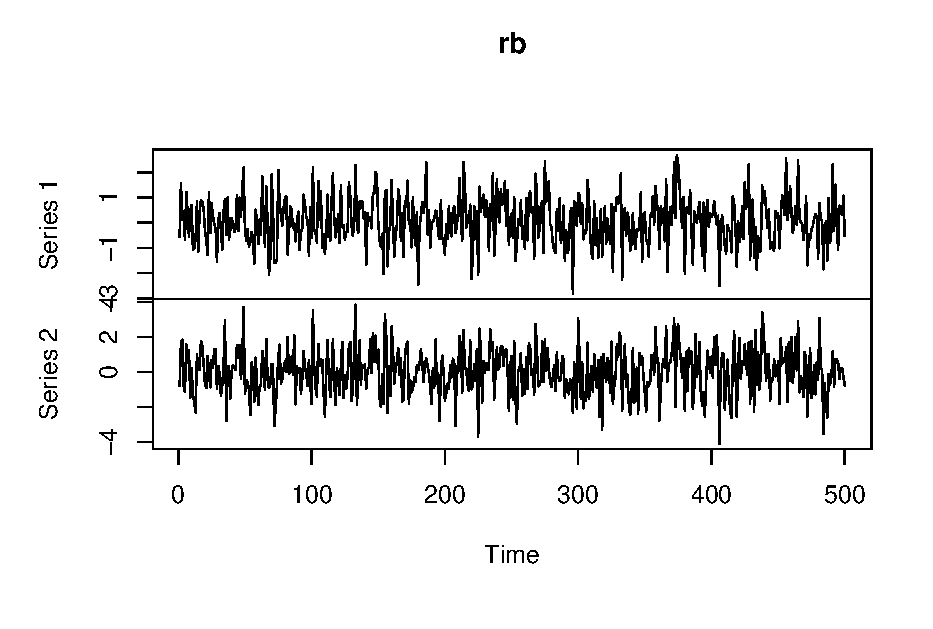
\includegraphics[scale=0.7]{graficos/rb_multi.pdf}
\end{figure}

\end{frame}

\begin{frame}{Modelos vetoriais autorregressivos}
	\begin{itemize}
		\item Considere $d$ séries de tempo $\{X_{j,t}: t \in \mathbb{Z}\}$, $j=1,\ldots, d$.
		\item Dizemos que estas séries definem um processo vetorial autorregressivo de ordem $p$, ou VAR(p), se, para todo $j=1,\ldots, d$ e $t\in \mathbb{Z}$:
	\end{itemize}
	\begin{equation*}
		\begin{aligned}
			X_{{\color{blue}j},t} &= a_{{\color{blue}j},0}  +\sum_{l=1}^p a_{{\color{blue}j},{\color{orange}1},l} X_{{\color{orange}1},t-l} + \sum_{l=1}^p a_{{\color{blue}j},{\color{orange}2},l} X_{{\color{orange}2},t-l}   +\ldots + \sum_{l=1}^p a_{{\color{blue}j},{\color{orange}d},l} X_{{\color{orange}d},t-l}  + \epsilon_{{\color{blue}j},t} \\
			&= a_{{\color{blue}j},0}  +{\color{orange}\sum_{k=1}^{d}}\sum_{l=1}^p a_{{\color{blue}j},{\color{orange}k},l} X_{{\color{orange}k},t-l} + \epsilon_{{\color{blue}j},t} \, ,
		\end{aligned}
	\end{equation*}
	onde $\boldsymbol{\epsilon}_t = (\epsilon_{1,t},\epsilon_{2,t},\ldots, \epsilon_{d,t})'$ é um ruído branco vetorial.
	\begin{itemize}
		\item No VAR(p), assim como no AR(p), evolução em cada uma das $d$ variáveis depende do que ocorreu nela mesma nos últimos $p$ períodos.
		\item Mas além disso, trajetória depende do que ocorreu nos últimos $p$ períodos {\color{orange}nas demais variáveis}.
		\item Série depende também de uma inovação $\epsilon_{j,t}$, imprevisível com base no passado, mas que pode estar contemporaneamente associada às demais inovações nas outras equações (choques comuns).
	\end{itemize}
\end{frame}

\begin{frame}{VAR(p) em notação vetorial}
	\begin{itemize}
		\item Um VAR(p) pode ser escrito, compactamente, em notação vetorial.
		\item De fato, definindo $\boldsymbol{X}_t = (X_{1,t},X_{2,t},\ldots, X_{d,t})'$, podemos escrever o sistema como
		
		\begin{equation*}
			\boldsymbol{X}_t = \boldsymbol{a}_0 + \boldsymbol{A}_1 \boldsymbol{X}_{t-1} + \boldsymbol{A}_2 \boldsymbol{X}_{t-2} + \ldots + \boldsymbol{A}_p \boldsymbol{X}_{t-p} + \boldsymbol{\epsilon}_t \, ,
		\end{equation*}
		onde
		$$\boldsymbol{a}_0 = \begin{bmatrix}
			a_{1,0} \\
			a_{2,0} \\
			\vdots \\
			a_{d,0}
		\end{bmatrix} \quad \quad \boldsymbol{A}_l = \begin{bmatrix}
			a_{1,1,l} & 	a_{1,2,l} & \ldots &	a_{1,d,l} \\
			a_{2,1,l} &  	a_{2,2,l}  &  \ldots & a_{2,d,l} \\
			\vdots & \vdots  & \ldots & \vdots  \\
			a_{d,1,l} & a_{d,2,l} & \ldots & a_{d,d,l}
		\end{bmatrix}$$ 
	\end{itemize}
\end{frame}
\begin{frame}{VAR(p) estacionário}
	\begin{itemize}
		\item Um VAR(p) é dito estacionário se o processo vetorial resultante é estacionário.
		\item Condição para estacionariedade do VAR(p) é que:
		
		$$ |z| \leq 1 \implies \operatorname{det}(\mathbb{I}_{d\times d} - \boldsymbol{A}_1 z - \boldsymbol{A}_2 z^2 \ldots -  \boldsymbol{A}_p z^p ) \neq 0$$
		\item Todas as raízes do polinômio $\phi(z) = \operatorname{det}(\mathbb{I}_{d\times d} - \boldsymbol{A}_1 z - \boldsymbol{A}_2 z^2 \ldots -  \boldsymbol{A}_p z^p )$ devem se encontrar fora do círculo unitário.
		\item Nesta aula, focaremos na estimação de VAR(p) estacionários.
		\begin{itemize}
			\item Portanto, cada uma das séries deverá estar devidamente estacionarizada. 
		\end{itemize}
	\end{itemize}
\end{frame}
\begin{frame}{Estimação do VAR(p)}
	\begin{itemize}
		\item 	Dado um painel com observações de $d$ séries durante $T$ períodos, $\{\boldsymbol{X}_{j,t}\}_{t=1}^T$, $j=1,\ldots, d$, como estimar os parâmetros de um VAR(p)?
		\item Maneira mais simples é estimar os parâmetros através de MQO, {\color{blue}equação a equação}.
		\item Isto é, estimamos os parâmetros da $j$-ésima equação resolvendo:
		
		$$\min_{b_{0,j}, \{b_{j,k,l}\}_{k,l}} \sum_{t=p+1}^T\left(\boldsymbol{X}_{j,t} - b_{0,j} - \sum_{k=1}^d \sum_{l=1}^p b_{j,k,l}X_{k,t-l}\right)^2$$
		\item Para cada equação, rodamos uma regressão com $T$ observações e $p\times d +1$ parâmetros.
	\end{itemize}

\end{frame}

\begin{frame}{SUR}
	\begin{itemize}
		\item A estimação dos parâmetros de um VAR por MQO, equação a equação, é potencialmente ineficiente.
					\item Isso se deve ao fato de que os choques em uma equação $j$, por serem (potencialmente) contemporaneamente correlacionados com os choques das demais equações, podem conter informação relevante para estimar os parâmetros de outras equações
		\begin{itemize}
		\item Erro em uma equação é informativo sobre a outra equação.
		\end{itemize}
		\item Seja $\hat \Sigma_0$ um estimador preliminar de $\mathbb{V}(\boldsymbol{\epsilon}_t)$.
		\begin{itemize}
			\item Por exemplo, estimador da variância-covariância com base nos resíduos do estimador de MQO equação a equação.
		\end{itemize}
		\item O estimador de \textit{seemingly unrelated regression} (SUR) dos parâmetros de um VAR propõe-se a estimar os parâmetros do sistema {\color{blue}conjuntamente}, minimizando:
	\end{itemize}		$$\min_{\boldsymbol{b}_0, \boldsymbol{B}_1,\ldots \boldsymbol{B}_p} \sum_{t=p+1}^T \left(\boldsymbol{X}_t - \boldsymbol{b}_0 -  \sum_{l=1}^p\boldsymbol{B}_l \boldsymbol{X}_{t-l}\right)' \hat \Sigma^{-1}_0 \left(\boldsymbol{X}_t - \boldsymbol{b}_0 -  \sum_{l=1}^p\boldsymbol{B}_l \boldsymbol{X}_{t-l}\right)$$
\end{frame}
\begin{frame}{Máxima verossimilhança condicional}
\begin{itemize}
	\item Sob a hipótese auxiliar:
	
	$$\boldsymbol{\epsilon}_t \overset{iid}{\sim} N(\boldsymbol{0}_{d\times 1}, \Sigma_0)$$
	podemos calcular a verossimilhança de $\boldsymbol{X}_{p+1},\ldots \boldsymbol{X}_{T}$, condicional a $\boldsymbol{X}_1,\ldots, \boldsymbol{X}_p$.
	\item Estimador de máxima verossimilhança condicional estima {\color{blue}simultaneamente} $\boldsymbol{a}_0$, os $\boldsymbol{A}_l$  e $\Sigma_0$.
\end{itemize}
\end{frame}
\begin{frame}{Relação entre os métodos de estimação}
\begin{itemize}
	\item Se o espaço de parâmetros é irrestrito, no sentido de que os parâmetros $\boldsymbol{a}_0$ e os $\boldsymbol{A}_l$ podem tomar qualquer valor real, os estimadores de MQO equação a equação, SUR, e máxima verossimilhança condicional são {\color{blue}numericamente iguais}.
	\item Se impomos restrições nos parâmetros $\boldsymbol{a}_0$ e os $\boldsymbol{A}_l$, estimador de MQO equação a equação é consistente, embora SUR e máxima verossimilhança condicional sejam mais eficientes.
	\item Se, além disso, impomos restrições na matriz ${\Sigma}_0$, os três estimadores são consistentes, mas máxima verossimilhança condicional é o mais eficiente.
\end{itemize}
\end{frame}

\begin{frame}{Selecionando a ordem $p$ de um VAR}
	\begin{itemize}
		\item Para selecionar a ordem $p$ de um VAR, podemos adotar generalizações multivariadas dos critérios de informação vistos para modelos univariados:
		
		$$\text{AIC}(p) = \operatorname{ln}(\operatorname{det}(\hat\Sigma(p))) + \frac{2}{T}(d^2 p + d)\, ,$$
						$$\text{HQ}(p) = \operatorname{ln}(\operatorname{det}(\hat\Sigma(p))) + \frac{2 \log \log(T)}{T}(d^2 p + d)\, ,$$
				$$\text{SC}(p) = \operatorname{ln}(\operatorname{det}(\hat\Sigma(p))) + \frac{\log(T)}{T}(d^2 p + d)\, ,$$
	onde $\hat \Sigma(p)$ é a matriz de variância-covariância dos resíduos do modelo VAR estimado com $p$ defasagens. 
	\item Assim como no caso univariado, no cálculo dos diferentes $\hat \Sigma(p)$, usamos os resíduos dos mesmos $T-\operatorname{p}_{max}$ períodos, onde $\operatorname{p}_{max}$ é a ordem máxima a se testar.
	\item Métodos oferecem aproximações ao erro quadrático médio de previsão um passo à frente, corrigidas do viés induzido por \textit{overfitting}.
	\end{itemize}
\end{frame}

\begin{frame}{Testando a inclusão de defasagens}
\begin{itemize}
	\item Partindo de um VAR(p), podemos testar se há necessidade de incluir a $p$-ésima defasagem.
	\item Especificamente, gostaríamos de testar.
	\begin{equation}
		H_0: \boldsymbol{A}_p = \boldsymbol{0}_{d \times d} \quad H_1:  \boldsymbol{A}_p \neq \boldsymbol{0}_{d \times d}
	\end{equation} 
	\item Teste pode ser conduzido através da estatística de razão de verossimilhança.
	\begin{equation}
		\operatorname{LR} = 2\cdot(\hat{L}_{p} - \hat{L}_{p-1})
	\end{equation}
	onde $\hat{L}_j$ é a log-verossimilhança maximizada do estimador de máxima verossimilhança condicional, do modelo que inclui $j$ defasagens.
	\item Sob hipótese nula, com $T$ grande, estatística segue distribuição qui-quadrado com $d^2$ graus de liberdade.
\end{itemize}
\end{frame}

\begin{frame}{Diagnóstico dos resíduos}
	\begin{itemize}
		\item Escolhida uma ordem $p$ do VAR, podemos avaliar o comportamento dos erros.
		\item Em particular, para $h \in \mathbb{N}$, podemos testar a hipótese nula:
		$$H_0: \operatorname{cov}(\boldsymbol{\epsilon}_{t}, \boldsymbol{\epsilon}_{t-j}) = \boldsymbol{0}_{d\times d}, \quad j=1,\ldots, h\, .$$
		usando um análogo vetorial do teste de Ljung-Box.
		\item A esse teste, damos o nome de {\color{blue}Portmanteau}.
		\item Também é possível estudar a normalidade conjunta dos erros, através de um análogo vetorial do teste de Jarque-Bera.
		\begin{itemize}
			\item Preocupação usualmente secundária. Normalidade garante que o MLE condicional domine outros estimadores condicionais, para além do MQO equação a equação e SUR. Também é importante na construção de intervalos de predição, assim como nos ARMA.
		\end{itemize}
	\end{itemize}
\end{frame}

\begin{frame}{Inclusão de componentes determinísticos}
	\begin{itemize}
		\item No modelo VAR apresentado, incluímos tão somente um intercepto entre os componentes determinísticos.
		\item Para  séries \textit{trend stationary}, devemos fazer o \textit{detrending} dos dados para a estimação do VAR estacionário.
		\item Se todas as séries apresentam tendência, um jeito mais eficiente de fazer isso é estimar conjuntamente a tendência ao VAR, ajustando o modelo:
		
			\begin{equation*}
			\boldsymbol{X}_t = \boldsymbol{a}_0 +\boldsymbol{a}_1 t + \boldsymbol{A}_1 \boldsymbol{X}_{t-1} + \boldsymbol{A}_2 \boldsymbol{X}_{t-2} + \ldots + \boldsymbol{A}_p \boldsymbol{X}_{t-p} + \boldsymbol{\epsilon}_t \, ,
		\end{equation*}
		
		\item Se há evidência de sazonalidade nas séries, podemos ajustar o VAR incluindo um conjunto de \textit{dummies} sazonais.
			\begin{equation*}
			\boldsymbol{X}_t = \boldsymbol{a}_0 +\boldsymbol{\gamma} \boldsymbol{d}_t + \boldsymbol{A}_1 \boldsymbol{X}_{t-1} + \boldsymbol{A}_2 \boldsymbol{X}_{t-2} + \ldots + \boldsymbol{A}_p \boldsymbol{X}_{t-p} + \boldsymbol{\epsilon}_t \, ,
		\end{equation*}
	\end{itemize}
\end{frame}

\begin{frame}{Previsão fora da amostra}
	\begin{itemize}
		\item Assim como nos modelos ARMA, a previsão em um modelo VAR se faz de maneira recursiva.
		\item Dados estimadores dos parâmetros do VAR,  previsão um passo à frente de $\boldsymbol{X}_{T+1}$ é dada por:
		
		$$\hat{\boldsymbol{X}}_{T+1} = \hat{\boldsymbol{a}}_0 +  \hat{\boldsymbol{A}}_1 \boldsymbol{X}_{T} + \hat{\boldsymbol{A}}_2 \boldsymbol{X}_{T-1} + \ldots + \ \hat{\boldsymbol{A}}_p \boldsymbol{X}_{T+1-P}  $$
		\item A previsão dois passos à frente é dada por: 
		
		$$\hat{\boldsymbol{X}}_{T+2} = \hat{\boldsymbol{a}}_0 +  \hat{\boldsymbol{A}}_1 {\color{red}\hat{\boldsymbol{X}}_{T+1} }+ \hat{\boldsymbol{A}}_2 \boldsymbol{X}_{T} + \ldots + \ \hat{\boldsymbol{A}}_p \boldsymbol{X}_{T+2-P}  \, ,$$
		e assim recursivamente.
		\item Previsões do VAR estacionário convergem para média incondicional estimada do processo:
		
		$$\lim_{h \to \infty }\hat{\boldsymbol{X}}_{T+h} = (\mathbb{I}-  \hat{\boldsymbol{A}}_1 -  \hat{\boldsymbol{A}}_2 \ldots -  \hat{\boldsymbol{A}}_p )^{-1}\hat{\boldsymbol{a}}_0 $$
	\end{itemize}
\end{frame}


\begin{frame}{Previsão \textit{online}}
\begin{itemize}
	\item Em diversas situações, a previsão em tempo real ocorre num cenário em que as divulgações dos valores mais recentes das variáveis ocorrem com defasagem no tempo.
	\begin{itemize}
		\item Dados para taxa inflação em $T+1$ são divulgados em um certo dia do mês $T+2$, enquanto dados da SELIC média de um mês podem ser obtidas antes, a depender do calendário do COPOM.
	\end{itemize}
	\item Nessas janelas intermediárias, em que alguns dados de $T+1$ já foram divulgados, mas faltam outros, é interessante entender como calcular as previsões para as variáveis que ainda não foram divulgadas para $T+1$, mas incorporando {\color{blue}toda} a informação disponível
	\begin{itemize}
		\item Se as defasagens entre divulgações forem muito longas e com um padrão bem-definido, uma possível solução, do ponto de vista preditivo, é trabalhar com as variáveis que saem muito antes de modo adiantado, i.e. incluímos a variável adiantada (em $t+1$) entre os $\boldsymbol{X}_t$ no modelo VAR. 
	\begin{itemize}
		\item No entanto, essa estratégia é menos útil quando o calendário de divulgações é mais irregular e com menos intervalos entre divulgações.
		\item Além disso, defasar algumas séries pode complicar a interpretação dos resultados das estimações.
	\end{itemize}
\end{itemize}
\end{itemize}
\end{frame}
\begin{frame}{Previsão \textit{online} e \textit{nowcasting}}
\begin{itemize}
	\item A alternativa para os cenários com divulgação irregular, que mantém a interpretabilidade dos coeficientes, consiste em realizar um procedimento conhecido como \textit{nowcasting}.
	\item Formalmente, suponha que podemos dividir o VAR em dois conjuntos de variáveis $\boldsymbol{X}_t = [{\color{blue}\boldsymbol{X}_{t}^e}, {\color{orange}\boldsymbol{X}_{t}^l}]$.
	\begin{itemize}
		\item Para as variáveis em $\boldsymbol{X}_{t}^e$, observamos os dados {\color{blue}até $T+1$}.
				\item Para as variáveis em $\boldsymbol{X}_{t}^l$, observamos os dados {\color{orange}até $T$}.
	\end{itemize}
	\item Sejam $\hat{\boldsymbol{a}_0}$, $\{\hat{\boldsymbol{A}_k}\}_{k=1}^p$ e $\hat{\Sigma}_0$ estimadores dos parâmetros do VAR com base em dados \textbf{até $T$}.
	\begin{itemize}
		\item Para esse conjunto de dados, não faltam informações para resolver o problema de otimização que produz o estimador.
	\end{itemize}
	\item Ideia é incorporar na projeção de $\boldsymbol{X}_{t}^l$ nossa melhor projeção para $\boldsymbol{\epsilon}^l_{T+1}$.
	\begin{itemize}
		\item Quando não temos dados de $T+1$, sabemos que nossa melhor projeção para esse termo é $\boldsymbol{0}$, visto que se trata de um ruído branco.
		\item No entanto, conhecimento de  $\boldsymbol{X}_{T+1}^e$ é possivelmente informativo sobre ruído branco, visto que há potencial correlação contemporânea nestes.
	\end{itemize} 
\end{itemize}
\end{frame}

\begin{frame}{\textit{Nowcasting}}
\begin{itemize}
 	\item Possível mostrar que melhor projeção (linear) para $\boldsymbol{\epsilon}^l_{T+1}$ com base no conhecimento do passado e $\boldsymbol{X}_{T+1}^e$ é:
 	$$ \boldsymbol{s}^l_{T+1} =   \Sigma_{l,e}\Sigma_{e,e}^{-1} \boldsymbol{\epsilon}_{T+1}^{e}$$
 	onde $\Sigma_{e,e} = \mathbb{V}[\boldsymbol{\epsilon}_t^e]$ e  $\Sigma_{l,e} = \operatorname{cov}[\boldsymbol{\epsilon}_t^l,\boldsymbol{\epsilon}_t^e]$.
 	\item Ideia é estimar $\boldsymbol{s}^l_{T+1}$ como:
 	$$\small \hat{\boldsymbol{s}}^l_{T+1} = \hat{\Sigma}_{0,l,e}\hat{\Sigma}_{0,e,e}^{-1}(\boldsymbol{X}^{e}_{T+1}-\hat{\boldsymbol{X}^{e}}_{T+1|T}),$$
 	onde $\hat{\boldsymbol{X}^{e}}_{T+1|T}$ é a projeção usual do VAR com dados até $T$, para $T+1$.
 	 \item Projetamos $\boldsymbol{X}^l_{T+1}$ como: 
 		$$\hat{\boldsymbol{X}}_{T+1}^l = \hat{\boldsymbol{X}^{l}}_{T+1|T} + \hat{\boldsymbol{s}}^l_{T+1}  $$
 		 	\item $\hat{\boldsymbol{s}}^l_{T+1}$ é o {\color{blue}ganho informacional} da divulgação adiantada de $e$.
 	\item Projeções para o horizonte longo são feitas de forma recursiva, usando $\hat{\boldsymbol{X}}_{T+1}^l $ e ${\boldsymbol{X}}_{T+1}^e $ para $T+1$.

\end{itemize}
\end{frame}

\begin{transitionframe}
	\centering	{\Huge Conceitos de interrelação para processos multivariados}
\end{transitionframe}

\begin{frame}{Distribuições conjuntas de processos vetoriais }
	\begin{itemize}
		\item Seja $\{\boldsymbol{Z}_t\}_{t \in \mathbb{Z}}$ um processo vetorial de interesse.
		\item A densidade conjunta numa janela  $\{\boldsymbol{Z}_t\}_{t =1}^T$, condicional a um valor inicial $\boldsymbol{Z}_0$, fatora-se como:
		
		$$f[(\boldsymbol{Z}_t)_{t=1}^T|Z_0] = \prod_{t=1}^T f[\boldsymbol{Z}_t|\mathcal{Z}_{t-1}]\, ,$$
		onde $\mathcal{Z}_{t-1} = (\boldsymbol{Z}_0, \boldsymbol{Z}_1,\ldots, \boldsymbol{Z}_{t-1})$.
	\end{itemize}
\end{frame}

\begin{frame}{Causalidade de Granger}
	\begin{itemize}
		\item Particione $\boldsymbol{Z}_t$ em dois conjuntos de variáveis, $\boldsymbol{Z}^1_t$ e $\boldsymbol{Z}^2_t$, com $d_1 + d_2 = d$.
		\item Dizemos que $\boldsymbol{Z}^2_t$ {\color{blue}não Granger causa} $\boldsymbol{Z}^1_t$ se:
		
		$$f(\boldsymbol{Z}^1_t|\mathcal{Z}_{t-1}) = f(\boldsymbol{Z}^1_t|\mathcal{Z}^1_{t-1}) \,,$$
		onde $\mathcal{Z}_{t-1}^1 = (\boldsymbol{Z}_0^1, \boldsymbol{Z}_1^1,\ldots, \boldsymbol{Z}_{t-1}^1)$.
		\item $\boldsymbol{Z}^2_t$ {\color{blue}não Granger causa} $\boldsymbol{Z}^1_t$ se defasagens de $\boldsymbol{Z}^2_t$ não são informativas sobre $\boldsymbol{Z}^1_t$.
		\begin{itemize}
			\item {\color{red}Conceito preditivo}, e não causal (no sentido econométrico do termo), embora o termo causalidade esteja no nome.
		\end{itemize}
		\item Em um modelo VAR(p) para $\boldsymbol{Z}_t$, onde $\boldsymbol{A}_l = \begin{bmatrix}
		\boldsymbol{A}_{l,1,1} & 	\boldsymbol{A}_{l,1,2} \\
				\boldsymbol{A}_{l,2,1} & 	\boldsymbol{A}_{l,2,2} \\
		\end{bmatrix}$,
		nula de que $\boldsymbol{Z}^2_t$  não Granger causa  $\boldsymbol{Z}^1_t$  é equivalente a:
		$$H_0: 	\boldsymbol{A}_{l,1,2} = \boldsymbol{0}_{d_1\times d_2}, \quad l =1,\ldots p\, .$$
	\end{itemize}
\end{frame}

\begin{frame}{Causalidade de Granger, causalidade contemporânea e exogeneidade Fraca}
\begin{itemize}
	\item Conceito de causalidade de Granger nos diz que conhecimento do passado de $\boldsymbol{Z}^2_t$ não é informativo sobre $\boldsymbol{Z}^1_t$ contemporâneo.
	\item Note que não falamos nada sobre conhecimento \textbf{contemporâneo} de $\boldsymbol{Z}^2_t$ ser informativo sobre   $\boldsymbol{Z}^1_t$ contemporâneo.
	\begin{itemize}
		\item De fato, num VAR, $\boldsymbol{Z}^2_t$ é no geral contemporanemanete informativo sobre  $\boldsymbol{Z}^1_t$ por conta das correlações em $\mathbb{V}(\boldsymbol{\epsilon}_t)$ diferentes de zero.
		\item No VAR, é possível testar essas relações contemporâneas olhando-se para as entradas de $\mathbb{V}(\boldsymbol{\epsilon}_t)$ ({\color{blue}``causalidade'' contemporânea}; também um conceito preditivo). 
		\begin{itemize}
			\item 	Nula de não causalidade contemporânea é que coeficiente do melhor preditor linear de $\boldsymbol{\epsilon}_{t}^1$ em $\boldsymbol{\epsilon}_{t}^2$ é zero, i.e. $\operatorname{cov}(\boldsymbol{\epsilon}_t^1, \boldsymbol{\epsilon}_t^2)\mathbb{V}[\boldsymbol{\epsilon}_t^2]^{-1} = \boldsymbol{0}_{d_1 \times d_2}$.
		\end{itemize}
	
	\end{itemize}
	\item Um conceito relacionado, embora diferente da causalidade de Granger, diz respeito à modelagem da distribuição de $\boldsymbol{Z}^2_t$ ser importante, do ponto de vista estatístico, na estimação do modelo para $\boldsymbol{Z}^1_t$.
	\item A esse conceito damos o nome de {\color{blue}exogeneidade fraca}.
\end{itemize}
\end{frame}
\begin{frame}{Modelo condicional e exogeneidade fraca}
	\begin{itemize}
		\item Formalmente, um modelo é uma parametrização da distribuição condicional  $f[\boldsymbol{Z}_t|\mathcal{Z}_{t-1}] = f[\boldsymbol{Z}_t|\mathcal{Z}_{t-1};\theta_0] $, onde $\theta_0 \in \Theta$ é um parâmetro desconhecido, que toma algum valor em $\Theta$.
		
		\item Note que sempre podemos escrever, usando a regra de Bayes:
			$$\small f[(\boldsymbol{Z}_t)_{t=1}^T|Z_0;\theta_0] = \prod_{t=1}^T f[\boldsymbol{Z}_t|\mathcal{Z}_{t-1};\theta_0] = \prod_{t=1}^T f[\boldsymbol{Z}_t^1|\boldsymbol{Z}^2_t,\mathcal{Z}_{t-1};\theta_0] f[\boldsymbol{Z}_t^2|\mathcal{Z}_{t-1};\theta_0] \, ,$$
		\item Nesse contexto, um subconjunto $\psi$ dos parâmetros $\theta_0$ é dito {\color{blue}fracamente exógeno com respeito a $\boldsymbol{Z}^2_t$} se podemos reescrever:
		$$f[\boldsymbol{Z}_t^1|\boldsymbol{Z}^2_t,\mathcal{Z}_{t-1};\theta_0] f[\boldsymbol{Z}_t^2|\mathcal{Z}_{t-1};\theta_0]  = f[\boldsymbol{Z}_t^1|\boldsymbol{Z}^2_t,\mathcal{Z}_{t-1};\lambda_1] f[\boldsymbol{Z}_t^2|\mathcal{Z}_{t-1};\lambda_2]  $$
		onde $\psi$ é  função somente de $\lambda_1$, e $\lambda_1$ e $\lambda_2$ podem variar {\color{blue}livremente}.
		\begin{itemize}
			\item No caso, não há perda de informação relevante em estimar $\psi$ somente considerando o modelo $\boldsymbol{Z}_t^1|\boldsymbol{Z}^2_t,\mathcal{Z}_{t-1}$, tratando $\boldsymbol{Z}^2_t$ como fixo.


		\end{itemize}
	\end{itemize}
\end{frame}
\begin{frame}{Exogeneidade fraca no VaR(p)}
\begin{itemize}
 			\item Se $\boldsymbol{Z}_t$ segue um VAR(p) e nosso interesse consiste em estudar a evolução de $\boldsymbol{Z}^1_t$ no tempo, exogeneidade fraca implica que não há perda de eficiência estatística em estimar o modelo que trata $\boldsymbol{Z}^2_t$ como uma {\color{red}variável externa} no modelo:
	$$\boldsymbol{Z}^1_t = \boldsymbol{b}_0  + \sum_{j=1}^p \boldsymbol{B}_j \boldsymbol{Z}^1_{t-j} + {\color{red}\sum_{l={\color{magenta}0}}^p \boldsymbol{C}_l \boldsymbol{Z}^2_{t-l}} + \boldsymbol{v}^1_t$$
	\begin{itemize}
		\item Se os coeficientes do modelo VAR(p) original para $\boldsymbol{Z}_t$ são irrestritos, então um subconjunto de variáveis $\boldsymbol{Z}^2_t$ sempre será fracamente exógeno.
	\end{itemize}
	\item Note, entretanto, que se formos usar a equação acima para previsão, precisaríamos ter projeções para trajetória de $\boldsymbol{Z}^2_t$ fora da amostra.

	\begin{itemize}
		\item Será que poderíamos usar projeções externas para $\boldsymbol{Z}^2_t$, por exemplo aquelas obtidas com base na estimação de um modelo com dados históricos de  $\boldsymbol{Z}^2_t$  ou mesmo aquelas divulgadas por um órgão externo, de maneira estatisticamente consistente?
		\begin{itemize}
			\item Esse é o conceito de \textbf{exogeneidade forte} que estudaremos agora. 
		\end{itemize}
	\end{itemize}
\end{itemize}
\end{frame}

\begin{frame}{Exogeneidade forte}
	\begin{itemize}
		\item O conceito de exogeneidade fraca nos diz que, para estimar $\psi$, não há perda de informação em considerar o modelo para $\boldsymbol{Z}_t^1|\boldsymbol{Z}^2_t,\mathcal{Z}_{t-1}$.
		\item Se formos realizar previsões para $\boldsymbol{Z}_{T+h}^1$ com base nesse  modelo, no entanto, vamos precisar de projeções para $\boldsymbol{Z}^2_{T+h}$.
		\item Podemos fazer isso imputando $\boldsymbol{Z}^2_{T+h}$ com base nas projeções de um modelo para $\boldsymbol{Z}^2_{T+h}$ com base somente no seu passado?
		\begin{itemize}
			\item Isso só faz sentido em termos estatístico-preditivos se $\boldsymbol{Z}^1_{T+h}$ \textbf{não Granger causa} $\boldsymbol{Z}^2_{T+h}$.
			\item Nesse caso, podemos modelar $\boldsymbol{Z}^2_{T+h}$ externamente e somente incluir suas projeções futuras no modelo para $\boldsymbol{Z}_t^1|\boldsymbol{Z}^2_t,\mathcal{Z}_{t-1}$.
		\end{itemize}
		\item Exogeneidade fraca de $\boldsymbol{Z}^2_t$ com respeito a $\psi$ + não causalidade de Granger $\boldsymbol{Z}^1_t$ sobre $\boldsymbol{Z}^2_t$: $\boldsymbol{Z}^2_t$ é {\color{blue}fortemente exógeno} com respeito a $\psi$.
	\end{itemize}
\end{frame}

\begin{frame}{Análise contrafactual e super exogeneidade}
\begin{itemize}
	\item Retorne à fatoração da densidade conjunta:
	$$f[\boldsymbol{Z}_t|\mathcal{Z}_{t-1};\theta_0]  = f[\boldsymbol{Z}_t^1|\boldsymbol{Z}^2_t,\mathcal{Z}_{t-1};\lambda_1] f[\boldsymbol{Z}_t^2|\mathcal{Z}_{t-1};\lambda_2]$$
	\item Essa fatoração, nos sugere um método para avaliar intervenções alternativas em $\boldsymbol{Z}^t_2$, que aqui são medidas por mudanças na distribuição $\boldsymbol{Z}_t^2|\mathcal{Z}_{t-1}$.
	\begin{itemize}
		\item Se $\boldsymbol{Z}_t^2$ é a taxa de juros e $\boldsymbol{Z}_t^1$ compila inflação e taxa de desemprego, qual seria o comportamento da taxa de juros sobre uma regra de decisão alternativa?
	\end{itemize} 
	\item Formalmente, a avaliação de políticas alternativas (contrafactuais) com base na estimação de $\hat \lambda_1$ só será válida sobre um requerimento adicional à exogeneidade fraca, denominado \textbf{invariância}.
	\begin{itemize}
		\item $\boldsymbol{Z}_t^1|\boldsymbol{Z}^2_t,\mathcal{Z}_{t-1}$ é invariante se modelo e seu parâmetro para $f[\boldsymbol{Z}_t^1|\boldsymbol{Z}^2_t,\mathcal{Z}_{t-1};\lambda_1]$ não mudam sob distribuições alternativas para $\boldsymbol{Z}_t^2|\mathcal{Z}_{t-1}$.
	\end{itemize}
	\item Exogeneidade fraca + invariância: {\color{blue}superexogeneidade} com respeito a um parâmetro.
\end{itemize}
\end{frame}



\begin{frame}{Invariância e crítica de Lucas}
	\begin{itemize}
		\item Num VAR(p) de inflação, desemprego e taxa de juros, a hipótese de invariância para  avaliação do efeito contrafactual de regra de juros alternativas parece razoável?
		\item A {\color{blue}crítica clássica de Lucas} sugere que, na medida em que as decisões de produção e preço de uma economia são tomadas por agentes racionais que levam em conta expectativas acerca do regime em questão, a resposta é \textbf{não}.
		\item Nesse caso, os parâmetros do VAR(p) em questão são funções complicadas dos parâmetros fundamentais da Economia (preferências, parâmetros da função de produção e política econômica), de modo que existe uma relação complicada entre os parâmetros de equações diferentes de um VAR(p).
		\begin{itemize}
			\item Não podemos simplesmente alterar uma das equações do modelo, mantendo as demais fixas nos valores estimados.
			\item Além disso, note que as equações do modelo, a princípio, também não são necessariamente funções política passíveis de modificação, e sim objetos de equilíbrio.
		\end{itemize}
		\end{itemize}
\end{frame}
\begin{frame}{Alternativas à crítica de Lucas}
\begin{itemize}
	\item A crítica de Lucas ensejou duas tradições na macroeconometria.
	\item A tradição de DSGE busca partir de modelos econômicos estocásticos microfundamentados e completamente especificados, e derivar um VAR(p) a partir das primitivas  do modelo econômico e de hipóteses de equilíbrio do sistema.
		\item Formalmente, o VAR(p) resultante se escreve nesses casos como 
	\begin{equation*}
		\boldsymbol{Z}_t = \boldsymbol{a}_0(\xi)+ \boldsymbol{A}_1(\xi) \boldsymbol{Z}_{t-1} + \boldsymbol{A}_2(\xi) \boldsymbol{Z}_{t-2} + \ldots + \boldsymbol{A}_p(\xi) \boldsymbol{Z}_{t-p} + \boldsymbol{\epsilon}_t(\xi) \, ,
	\end{equation*}
	onde $\xi$ são os parâmetros fundamentais (preferências, tecnologia, política fiscal e monetária etc.), e tanto os  choques como $\boldsymbol{A}_l$ são funções complicadas desses parâmetros que emergem do equilíbrio do sistema.
	\item Ideia é estimar $\xi$ indiretamente a partir do VAR(p), e realizar os contrafactuais variando-se $\xi$.
	\begin{itemize}
		\item Dificuldades de identificação, estimação e inferência. 
		\item Além disso, método depende muito da correta especificação do modelo.
	\end{itemize}
	
\end{itemize}
\end{frame}
\begin{frame}{VAR (semi)estrutural}
	\begin{itemize}
	 	\item Uma segunda tradição busca postular modelos que, partindo da teoria econômica, explicitem as relações causais entre as variáveis, embora sejam agnósticos sobre os microfundamentos específicos dos problemas.
	 	\begin{itemize}
	 		\item Diversos modelos econômicos postulam relações contemporâneas e extemporâneas entre desemprego, juros e inflação.
	 	\end{itemize}
	 	\item Definido o modelo, analisamos condições que garantam que sejamos capazes de avaliar o efeito de choques (surpresas) nas variáveis de política econômica sobre as demais variáveis, \textbf{no regime em questão}.
	 	\begin{itemize}
	 		\item Análise de natureza causal, embora não contrafactual (visto que mantemos o regime atual).
	 		\item Para análise contrafactual, precisamos de mais hipóteses, visto que não postulamos todos os microfundamentos como na abordagem DSGE.
	 	\end{itemize}
	 	\item Abordagem de VAR (semi)estrutural, que veremos mais à frente no curso.
	\end{itemize}
\end{frame}
%\appendix
%\begin{frame}{Referências}
%	\printbibliography
%\end{frame}
\end{document}

